\chapter[Capítulo 2. Background en problemas]{Background en problemas}

\section{Clasificación sobre flujos de datos}

Los sistemas tradicionales basados en el uso de memoria, entrenados de una forma fija mediante conjuntos de entrenamiento y los cuales generan modelos estáticos, no están
preparados para procesar los datos altamente detallados disponibles en procesos como, por ejemplo, el continuo análisis de datos generados por los sensores de una máquina que trabaja sin descanso, lo cual crea una gran cantidad de datos que ha de ser procesada de forma rápida con el fin de generar modelos predictivos consistentes
que se adapten a situaciones cambiantes y puedan reaccionar de forma rápida y eficaz a dichos cambios.

El Machine Learning extrae conocimiento en forma de modelos y patrones de unos datos de naturaleza cambiante. Hoy en día la generación de datos, gracias a las capacidades
tecnológicas de las que disfrutamos, se produce a altas velocidades, tanto es así, que se pone, en cuanto a velocidad, por delante del procesamiento de dichos datos, lo cual
quiere decir que generamos datos a mayor velocidad de lo que las capacidades computacionales que tenemos ahora mismo nos permiten procesarlos.\\
Desde este punto de vista, en estos casos conviene modelar los datos como flujos de datos transitorios en lugar de como tablas de datos persistentes.

\begin{figure}[H]
	\centering
	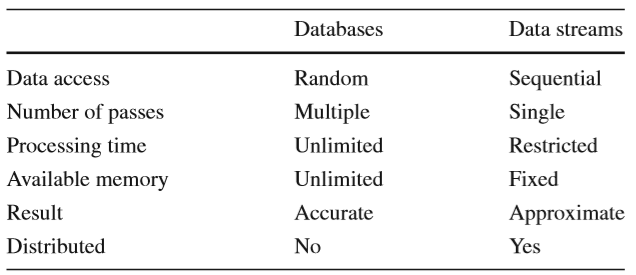
\includegraphics[width=0.9\textwidth]{imagenes/tabla1} 
	\caption{Resumen entre las diferencias principales entre el procesamiento estándar de una base de datos y el procesamiento de flujo de datos. \cite{ref1}}
\end{figure}



\subsection{Tipos de algoritmos para flujos de datos}

Existen dos tipos distintos de algoritmos que trabajan sobre flujos de datos:
\begin{itemize}
	\item \textbf{Insert-only model}: donde los datos entran al sistema de forma secuencial.
	\item \textbf{Insert-delete model}: donde los elementos que entran pueden ser eliminados o actualizados.
\end{itemize}

Desde el punto de vista de los sistemas de control de flujo de datos(DSMS), existen varios problemas que requieren técnicas de procesamiento no exactas para evaluar el flujo continuo de datos que requieren una cantidad ilimitada de memoria.

Estos algoritmos de procesamiento flujos de datos producen soluciones aproximadas dentro de un rango de error admisible para ciertas aplicaciones, con una alta probabilidad, relajando así las restricciones a la hora de obtener una solución exacta.

Los sistemas de control de flujos de datos han desarrollado un conjunto
de técnicas que almacenan resúmenes de datos compactos suficientes para resolver consultas. Estas aproximaciones requieren un equilibrio entre el accuracy y la cantidad de memoria usada para almacenar los resúmenes, con una restricción adicional de tiempo de procesado de los datos.


\subsection{Aproximación y aleatorización}

Dentro del marco del data streaming, como ya hemos dicho, está permitido ofrecer respuestas aproximadas dentro de un pequeño rango de error ($\epsilon$), con una pequeña probabilidad de fallo ($\delta$) para obtener respuestas con una probabilidad de que 1-$\delta$ se encuentre en el intervalo de radio $\epsilon$.

Los algoritmos que usan estas aproximacióon y aleatorización son referidos por dichos ($\epsilon$,$\delta$).\\
la idea consiste básicamente en mapear cada espacio grande de entrada en una sinopsis pequeña.\\
La aproximación y randomización han sido usadas en solventar problemas como minería de reglas de asociación, items frecuentes, k-means...


\subsection{Ventanas de tiempo}

Para la realización del cómputo estadístico referente al modelo de flujos, no nos interesa el total de los datos existentes, si no los más recientes, entendiendo que son los que mejor explican la situación a la que nos enfrentamos y pudiendo, de esta forma, deshacernos de grandes cantidades de datos que no nos son útiles.

Las técnicas más simples para este tipo de tratamiento de datos, utilizan una ventana deslizante de tamaño fijo, con un funcionmiento FIFO (first in fist out).

Definimos dos tipos de ventana deslizante:
\begin{itemize}
	\item \textbf{Basada en secuencia}: donde el tamaño de ventana queda definido por el número de observaciones del data set (tamaño fijo o variable en el tiempo).
	\item \textbf{Basada en marca de tiempo}: donde el tamaño de ventana está definido en términos de duración. Una ventana de este tipo de tamaño t consiste en todos los elementos cuya marca de tiempo
	se situa dentro del intervalo de tiempo t del actual periodo de tiempo.
\end{itemize}

El hecho de monitorizar, analizar y extraer conocimiento de flujos de datos de alta velocidad, puede hacer que existan diversos niveles de \textbf{granularidad} a la hora de 
almacenar los datos. Conforme más antiguos son los datos que disponemos, mayor granularidad requeriremos en la información (es decir, menor precisión). Cuanto más
reciente sean los datos, el grano ha de ser más fino, ya que requerimos más precisión al tratarlos debido a que son más importantes (este es llamado el\textbf{ modelo de ventana de tiempo inclinado}).

\subsubsection{Ejemplo de algoritmo de ventana de tiempo}

\textbf{AdWin-ADaptive sliding WINdow}: mantiene una ventana variable con respecto a los items recientemente vistos con la propiedad de que la ventana tiene un tamaño maximal
estadísticamente consistente con la hipótesis de que no haya habido un cambio en la media del valor dentro de la ventana. Un fragmento viejo de la ventana se desecha
si hay alguna evidencia de que tiene un valor distinto al del resto de la ventana.


\subsection{Muestreo}

El sampling (o muestreo) consiste en la selección del subconjunto de datos a analizar en intervalos periódicos, utilizado para calcular estadísticas del flujo (valores esperados).\\
Este tipo de técnicas reduce la cantidad de datos a procesar, por tanto, el coste computacional.\\
Como contra a su uso, podemos decir que pueden ser una fuente de errores, por ejemplo, en aplicaciones dedicadas a la detección de valores extremos o anomalías, ya que, a la hora de realizar el sampling podemos estar eliminando dichas instancias. El problema principal es obtener una muestra representativa.


Técnicas de muestreo:
\begin{itemize}
	\item \textbf{Random sampling}: muestreo aleatorio de los datos (todas las instancias con la misma probabilidad de ser escogidas).
	\item \textbf{Reservoir sampling}: consiste en mantener una muestra de tamaño K de reserva. A medida que fluyen los datos, cada nuevo elemento tiene una probabilidad k/n (donde n son los datos visualizados hasta el momento) de reemplazar un antiguo dato.
	\item \textbf{Load shedding}: elimina secuencias del flujo de datos cuando se producen cuellos de botellas en las capacidades de procesamiento.
\end{itemize}

\subsection{Sinopsis, bocetos y resúmenes}
A continuación describimos tres métodos de compactación de información para la generación de modelos sobre los ya comentados conjuntos de datos reducidos para data streaming:

\begin{itemize}
	\item \textbf{Sinopsis}: estructuras de datos compactas que resumen datos para su posterior consulta.
	\item \textbf{Data sketching}: herramienta de reducción de dimensionalidad. Usa proyecciones aleatorias de datos con cierta dimensión d a un espacio de cierto conjunto de dimensiones.
	\item \textbf{Data stream summary (by Cirnide and Muthukrishnan)}: usado para aproximaciones ($\epsilon$,$\delta$) para resolver consultas de rango, consultas puntuales y consultas innerproduct.
\end{itemize}





\subsection{Problemas en el aprendizaje sobre data streams}

El objetivo de la minería de datos es la habilidad de mantener de forma permanente un modelo de decisión preciso.
Este problema requiere algoritmos que se adapten a los datos conforme esten disponibles para poder aprender de ellos.
Además, los datos desactualizados han de ser olvidados para dejar de tenerlos en cuenta a la hora de crear el modelo, cosa que ha de ocurir en la presencia de 
información con una distribución no estacionaria presente. El aprendizaje en flujos de datos requiere por tanto algoritmos incrementales de aprendizaje que tengan en
cuenta el llamado "concept drift".

La solución a estos problemas requieren nuevas técnicas de muestreo y randomización, y nuevos algoritmos aproximados, incrementales y decrementales.
Algunas propiedades deseables para algoritmos de flujos de datos:
\begin{itemize}
	\item \textbf{Incrementalidad}
	\item \textbf{Aprendizaje online}
	\item \textbf{Tiempo constante de procesado de cada ejemplo}
	\item \textbf{Un solo escaneo sobre el conjunto de datos de training}
	\item \textbf{Tener en cuenta el concept drift}
\end{itemize}


Los algoritmos de aprendizaje incrementales y decrementales requieren una permanente actualización del modelo de decisión conforme llegan datos nuevos. Esta habilidad 
de actualizar el modelo mediante las propiedades de los nuevos datos es importante, pero no suficiente, ya que también es necesaria la habilidad de olvidar información
anticuada para dar un giro en el aprendizaje realizado, dejando de tener en cuenta los items antiguos: decremental learning.

Evidentemente existe una balanza entre la ganancia en rendimiento ofrecido por el algoritmo y la manutención de la característica de actualización de este, lo que hace que 
el cómputo realizado por el algoritmo sea más complejo. Ante esta balanza, con el fin de no acrecentar el cómputo, haciendo que el algoritmo decida de forma dinámica
qué información borrar y cuál no, surge la ya comentada técnica de ventana deslizante.

De forma general, es complicado asumir que, en el manejo de flujos de datos durante un largo tiempo, estemos tratando con datos acordes a una distribución de probabilidad
estacionaria. En sistemas complejos y en largos periodos de tiempo, debemos esperar cambios en la distribución de los items.

Una aproximación natural para estas tareas incrementales son los algoritmos de aprendizaje adaptativo, algoritmos incrementales que tienen en cuenta el concept drift.
El concept drift en sí, se refiere al cambio de concepto que sufren los datos a la largo del tiempo, cada vez con cierta permanencia mínima.
Hay algoritmos que implementan el olvido de información antigua teniendo en cuenta este cambio de concepto, lo que los hace mucho más precisos que los propios algoritmos
que realizan la eliminación de información en forma de tamaño de ventana prefijado.\\
Con el uso de los algoritmos de detección de concept drift podemos averiguar cuando y por qué ha cambiado el comportamiento del flujo de datos.\\
Estos algoritmos no poseen la información de mundo cerrado de la que disponen los algoritmos convencionales para el tratamiento de datos estáticos, si no que han de ser
capaces de adaptarse a un mundo abierto cambiante de datos para diferenciar entre cambio de concepto y ruido en los datos.

A la hora de evaluar los resultados en el contexto de los flujos de datos, es interesante tener en cuenta la evolución del acierto de nuestro algoritmo a lo largo del tiempo
con los cambios de concepto acaecidos.



\subsection{Requisitos y funcionamiento de flujos de datos}

A modo de resumen, planteamos los requisitos primordiales para la clasificación de data streams de la siguiente forma:
\begin{enumerate}
	\item Procesamiento de un ejemplo en cada instante de tiempo e inspección de este tan solo una vez.
	\item Limitado uso de memoria.
	\item Trabajo en un tiempo limitado.
	\item Estar listo para predecir en cualquier momento.
\end{enumerate}

De la misma forma, describimos el ciclo de clasificación para flujos de datos
\begin{enumerate}
	\item El algoritmo toma el siguiente ejemplo del flujo
	\item El algoritmo procesa el ejemplo actualizando sus estructuras de datos. En este punto no se ha de exceder los límites de memoria y ha de ser lo más rápido posible.
	\item El algoritmo está listo para aceptar el siguiente ejemplo.
\end{enumerate}

\begin{figure}[H]
	\centering
	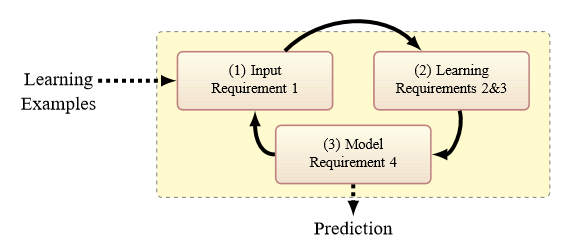
\includegraphics[width=1\textwidth]{imagenes/ccfd} 
	\caption{Ciclo de clasificación para flujos de datos junto con los requisitos utilizados en cada paso de los descritos anteriormente.}
\end{figure}

Para el procedimiento de evaluación de los algoritmos de aprendizaje, mientras que los modelos batch tradicionales utilizan un conjunto de datos de train y otro de 
test de reserva (holdout) para realizar dicha evaluación, en los algoritmos dedicados al data streaming se utiliza el método  Interleaved Test-Then-Train o Prequential,
mediante el cual cada una de las instancias que se reciben se utilizan como instancia de test para, posteriormente, usarla como nuevo dato de aprendizaje (train).
De esta forma no es necesario mantener un conjunto de datos de reserva exclusivo para validar, haciendo que el uso de los datos disponibles sea máximo, además
de que ayuda a crear una representación más visual de la evolución de la precisión del algoritmo a lo largo del tiempo.














\section{Clasificación ordinal y monotónica}

Comenzamos este apartado definiendo primeramente un par de conceptos básicos para adentrarnos de forma correcta en el significado
de la clasificación ordinal y monotónica: \cite{ref17}

\begin{itemize}
	\item \textbf{Principio de dominancia}: a mayor valor en atributos de una instancia, mayor será el
	valor de la clase a la que se asigna dicha instancia.
	Usando el termino de ''relación de dominancia'' decimos que una instancia x domina a
	otra instancia x' cuando cada una de las variables de entrada de x (atributos de x)
	son mayores o iguales que cada uno de los de x', se denota x$\geq$x' y por tanto
	x tendrá asignada una etiqueta de clase mayor que x'.
	\item \textbf{Función monótona}: una función es monótona si x$\geq$x' $\rightarrow$ h(x)$\ge$h(x') . Es decir, si x domina a x', la
	inferencia de clase de x ha de ser superior a la de x'.
\end{itemize}

Una vez definidos estos conceptos, podemos describir el sentido de la clasificación ordinal con restricciones monotónicas así como su diferencia con respecto a la clasificación ordinal simple:

\begin{itemize}
	\item La \textbf{clasificación ordinal con restricciones monotónicas} maneja conocimiento subyacente del
	problema sobre clases ordenadas, atributos ordenados y una relación monotónica entre
	la evaluación de los atributos de una instancia y la asignación de esta a una clase.
	\item Si no hay relación de monotonía en la asociación de una clase a una instancia, 
	pero las clases si poseen un orden, entonces se considera\textbf{ clasificación ordinal} simplemente.
\end{itemize}

Con las restricciones de monotonía presentes se puede trabajar con una amplia
variedad de funciones sin temor a que introduzcan más restricciones que 
la de monotonía: es posible hacer inferencia de la clase sobre todas las funciones
monótonas.\\
La clasificación monotónica puede ser directa (más habitaciones, precio mayor
de una casa), o inversa (más polución, precio menor de la casa).\\
Normalmente en problemas de clasificación monotónica reales, las restricciones
monotónicas son consideradas en un subconjunto de características del dataset, no en todos los atributos.

Ejemplos de uso de monotonicidad: \cite{ref15}
\begin{itemize}
	\item Comparación de dos compañías donde una domina sobre la otra en términos de
	todos los indicadores financieros. Debido a esto, la compañía dominante
	ha de tener una evaluación final superior a la compañía dominada. Un uso
	de esto, es la predicción de la calificación crediticia usada por los bancos.
	\item House pricing: el precio de una casa será superior cuantas más habitaciones
	posea, mejor sea la calidad del aire acondicionado y menor sea la polución
	en el ambiente.
\end{itemize}



\subsection{Restricciones monotónicas}

La motivación del uso de restricciones monotónicas viene dada por los siguientes aspectos:
\begin{itemize}
	\item El tamaño del espacio de la hipótesis es reducido, lo que facilita el
	proceso de aprendizaje. 
	\item Otras métricas además de la precisión, como la consistencia con respecto
	a estas restricciones, pueden ser usadas por los expertos para aceptar
	o rechazar el modelo. Estas técnicas de evaluación de restricciones
	monotónicas las veremos más adelante con el fin de poder evaluar 
	la consistencia de estas.
\end{itemize}

Las restricciones impuestas a continuación, son restricciones con respecto a la probabilidad de distribución en la generación de 
datos, además de imposiciones sobre la función de perdida bajo las cuales
el clasificador óptimo de Bayes es monótono.

\subsubsection{Dominancia estocástica}

El principio de dominancia no siempre
se aplica en la práctica de forma tan restrictiva, por lo que hemos de 
hablar en términos probabilísticos a la hora de referirnos a dichas
restricciones.

Decimos entonces que, siendo 'k' una de las posibles clases a tomar en el 
dominio por una instancia 'x', y siendo 'y' la etiqueta asignada a dicha
instancia 'x', si la restricción monótona nos dice que x$\ge$x', entonces
la dominancia estocástica nos dice que P(y$\le$k|x)$\le$P(y$\le$k|x').
Es decir, que la probabilidad de que el valor asignado (y) a la instancia 
dominante (x) sea mayor que cierto valor fijado de la clase (k), es mayor
que la probabilidad de que el valor asignado (y) a la instancia dominada(x')
sea mayor que ese mismo cierto valor de la clase fijado.

La relación de dominancia estocástica entre distribuciones se denota así:\\

%x \geq x' \Longrightarrow{P(y$|$x) \geq  P(y$|$x')} 

\begin{figure}[H]
	\centering
	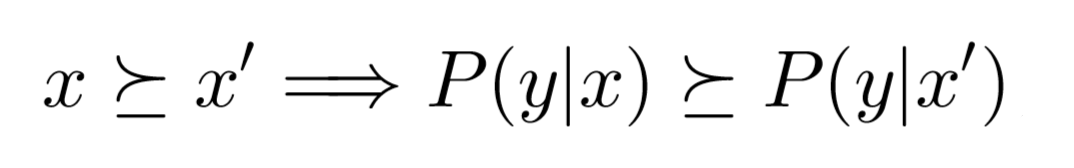
\includegraphics[width=0.4\textwidth]{imagenes/f1}
\end{figure}



Donde P(y$|$x) y P(y$|$x') denotan las distribuciones condicionales de la clase en x y x'. 

\subsubsection{Clasificador monótono de Bayes}

En el problema de clasificación el objetivo es encontrar el clasificador más
parecido al clasificador de Bayes, es decir, esta es nuestra función objetivo.
Sabiendo esto, se convierte en requisito el hecho de que este también aplique
las restricciones de monotonía que hemos enunciado. 

\textbf{Problema}: aunque la
distribución de probabilidad tiene restricciones monotónicas, el clasificador
de Bayes no siempre las mantiene.
Para solucionar este problema y mantener la monotonía en el clasificador de 
Bayes, han de imponerse las siguientes restricciones a la función de perdida
(L):

\begin{itemize}
	\item L(y,k+1)-L(y,k) $\ge$ L(y+1,k+1)-L(y+1,k) \\
	Esta característica de la función de pérdida es necesaria
	en la clasificación con restricciones monotónicas, si no no
	tendría sentido minimizar el riesgo dentro de la clase de las funciones monótonas.\\
	(Demostrado en \cite{ref17})
	\item La siguiente definición de convexidad es necesaria también para
	mantener la restricción de monotonía en el clasificador de Bayes:
		\begin{itemize}
			\item Siendo L(y,k) = c(y-k) (con c(0)=0)
			\item La función c(k) es convexa si, para todo k entre -(k-1) y (k-1):\\
			c(k) $\le$ (c(k-1)+c(k+1))/2
			\item El clasificador de Bayes es monótono si y solo si c(k) (que es
			la V-shaped loss function) es convexa.
		\end{itemize}
\end{itemize}


\subsection{Métodos de clasificación no paramétricos}

Los métodos no paramétricos son así llamados porque explotan la clase de todas las
funciones monótonas. Estos métodos no hacen ninguna asunción más sobre el modelo que la de 
las restricciones monotónicas.

\subsubsection{Aproximación Plug-In}

Pretenden \textbf{estimar la distribución condicional de la clase}. Provienen de la
clasificación isotónica (monótona creciente o decreciente)

Hemos de construir un método para estimar P(y$|$x), sabiendo que P(y$|$x) posee
dos ventajas:
\begin{enumerate}
	\item La distribución condicional permite la determinación de la predicción 
	óptima para cualquier función de pérdida.
	\item La distribución condicional mide la confianza de la predicción.
\end{enumerate}


\textbf{Problema de la clasificación binaria y la regresión isotónica.}

En la aproximación plug-in se propone usar un vector de estimadores de densidad
condicional p = (p1,....,pn), el cual es una regresión isotónica del vector de
etiquetas y = (y1,...,yn). Es decir, p nos da la probabilidad de que x 
pertenezca a cada una de las clases existentes en y.

Dicho vector p es la solución del problema: $\sum_{i=1}^n{(yi-pi)^2}$  sujeto a las restricciones de
monotonicidad (Xi$\ge$Xj $\rightarrow$ pi$\ge$pj). Por ello p minimiza el error cuadrático en 
el conjunto de los vectores monótonos p=(p1,..,pn) para cada x.

La elección de la función de error (función de perdida de error cuadrático)
parece ser arbitraria. Puede verse que haciendo uso de otras funciones
de perdida, se llega al mismo resultado.

La regresión isotónica es un problema de optimización cuadrática con 
restricciones lineales, por ello puede ser resuelta de forma eficiente con
la mayoría de los resolutores de optimización de propósito general.

\textbf{Problema multiclase.}

Está basado en la regresión isotónica multiclase y, la idea es descomponer el problema de K-clases en varios problemas binarios
y aplicar regresión isotónica a cada uno de los problemas.
Está demostrado que la descomposición del problema de estimación de 
probabilidad para el caso de multiclase, siempre forma una adecuada 
distribución de probabilidad, es decir, que siempre son no negativos
y la suma es igual a 1.


\subsubsection{Aproximación directa}

Consideramos la clasificación directa basada en la\textbf{ minimización del riesgo 
empírico} dentro de la clase de todas las funciones monótonas.\\
Aunque este tipo de funciones no se pueden describir con un número 
finito de parámetros, la minimización del riesgo puede realizarse debido a 
que solo estamos interesados en valores de funciones monótonas en ciertos
puntos, los incluidos en D (training set).

Una función monótona minimizando el riesgo empírico puede obtenerse resolviendo
el siguiente problema de optimización:

\begin{itemize}
	\item Minimizar: $\sum_{i=1}^n{L(y_i,d_i)}$.
	\item Teniendo en cuenta las restricciones de monotonía.
	\item Donde di son variables del problema (valores de la función monótona óptima
	en puntos de D)
\end{itemize}

El problema puede tener \textbf{otra interpretación} interesante: reetiquetar las
instancias para hacer el dataset monótono de forma que las etiquetas de las
instancias sean lo mas parecidas a las del conjunto original, donde esta 
similitud es medida en términos de la función de pérdida. Estas nuevas
etiquetas serán los nuevos valores óptimos de las variables di. 
Este reetiquetado puede realizarse en el proceso de preprocesamiento
y corresponde a la \textbf{corrección del error no paramétrico}.

Como el problema de clasificación no paramétrica se asimila al de la regresión
isotónica (exceptuando que ahora se considera una salida discreta), será llamado
ahora ''clasificación isotónica'' y su solución optima d\^ será llamada
''clasificación óptima de y''




\newpage

